
%(BEGIN_QUESTION)
% Copyright 2012, Tony R. Kuphaldt, released under the Creative Commons Attribution License (v 1.0)
% This means you may do almost anything with this work of mine, so long as you give me proper credit

A truck with a winch on the front is pulling a car up a steep hill.  The tension (pulling force) in the cable is 1000 pounds.  How many pounds is the horizontal component of this force that the truck has to resist with its brakes?  How many pounds is the vertical component of this force that the truck has to resist with its suspension (springs)?  Assume that the angle of the hill is 35$^{o}$ from level:

$$\includegraphics[width=15.5cm]{i02069x01.eps}$$

$F_{brakes}$ = \underbar{\hskip 50pt} lbs

\vskip 10pt

$F_{suspension}$ = \underbar{\hskip 50pt} lbs

\vskip 20pt \vbox{\hrule \hbox{\strut \vrule{} {\bf Suggestions for Socratic discussion} \vrule} \hrule}

\begin{itemize}
\item{} A technique highly recommended for word-problems is to {\it sketch a picture} of the problem and label elements of that picture with the given information.  Do this, and compare your sketch with those of your classmates.  How, specifically, does this aid your problem-solving?
\end{itemize}

\underbar{file i02069}
%(END_QUESTION)





%(BEGIN_ANSWER)

The truck's brakes must resist {\bf 819.15} pounds of horizontal force, to keep it from rolling in the direction of the slope.  The truck's suspension must bear {\bf 573.58} pounds of vertical force (in addition to the truck's own front-end weight).

%(END_ANSWER)





%(BEGIN_NOTES)


%INDEX% Mathematics review: trigonometric calculations

%(END_NOTES)


